%%%%%%%%%%%%%
\begin{figure}[h]
  \centering
    \subfigure[]{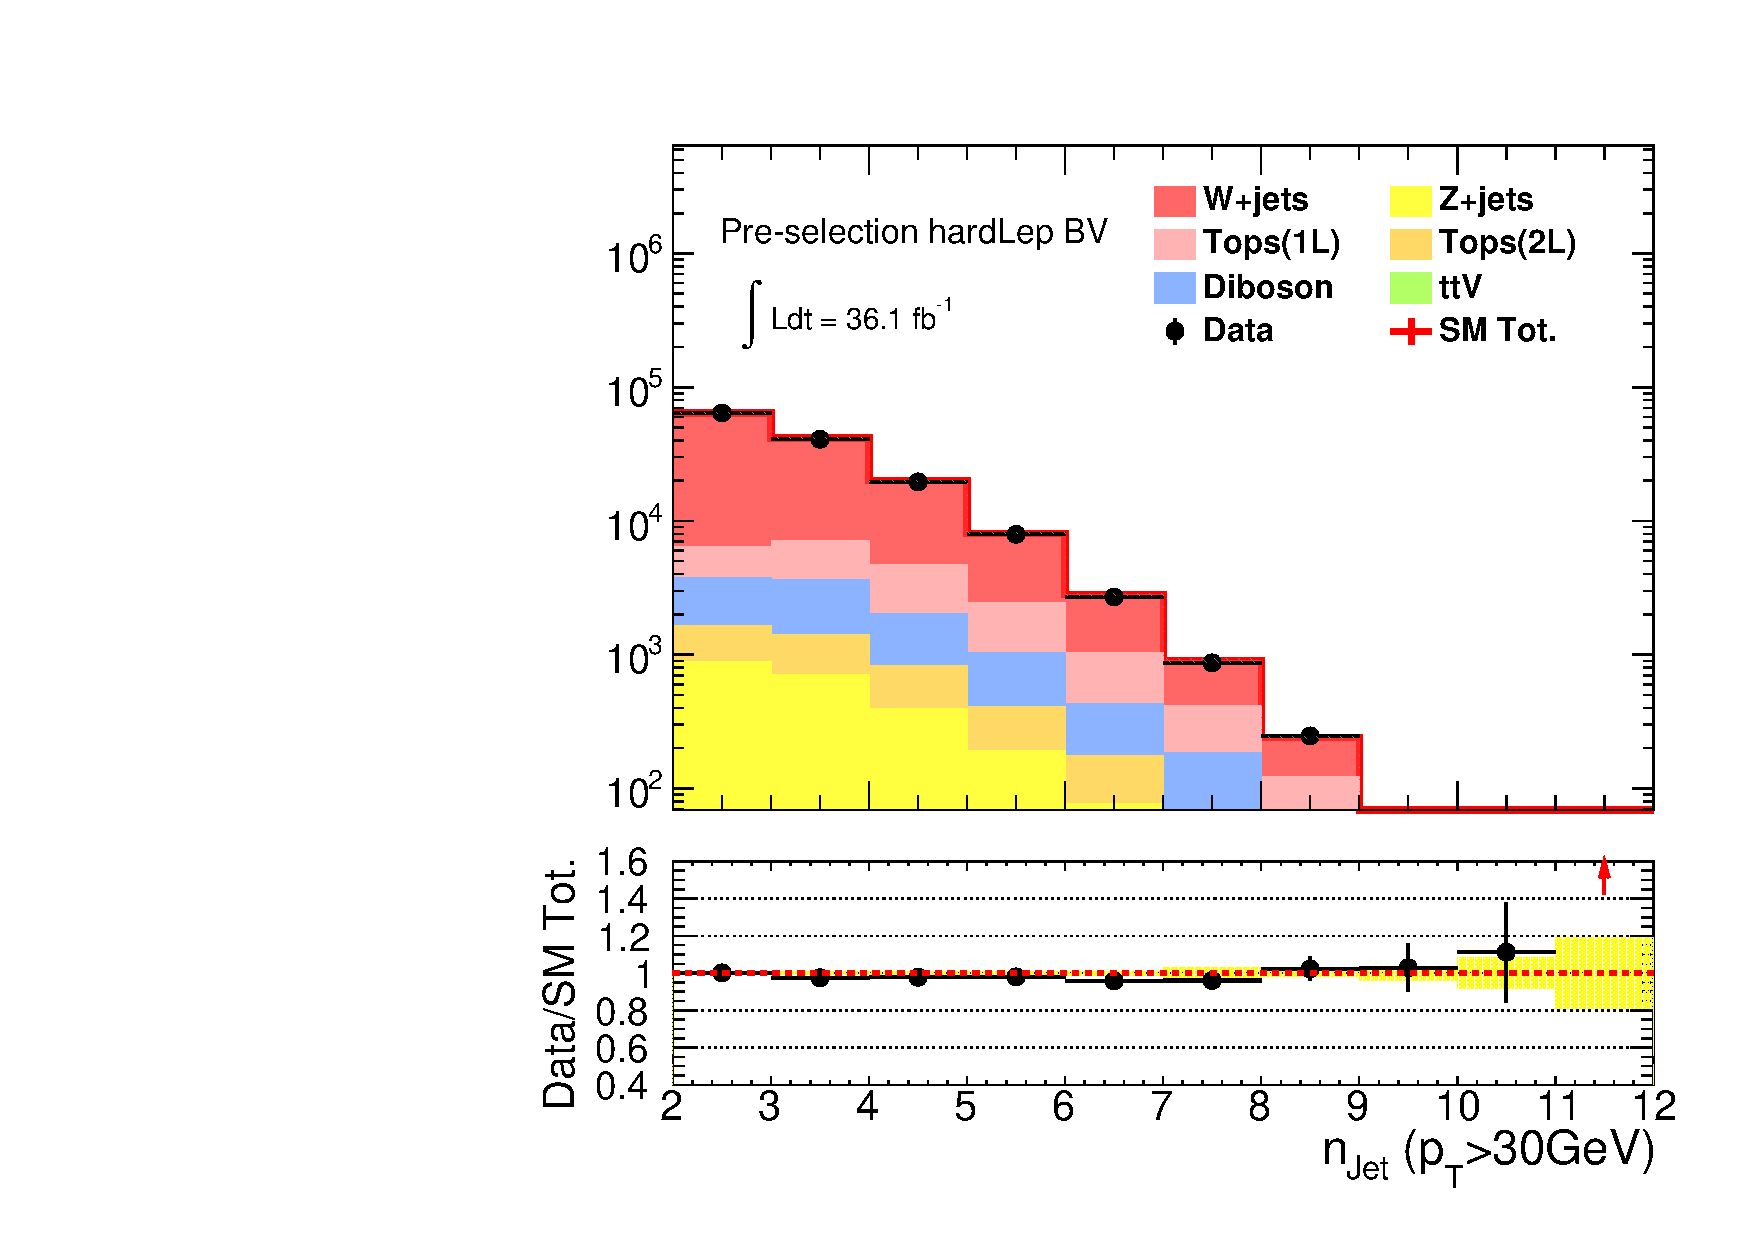
\includegraphics[width=0.48\textwidth]{figures/BGestimation/DataMCComparison/Preselection_hardLepBV/nJet30__Preselection_hardLepBV__rwgt_nJ007_ttPt007.pdf}}
    \subfigure[]{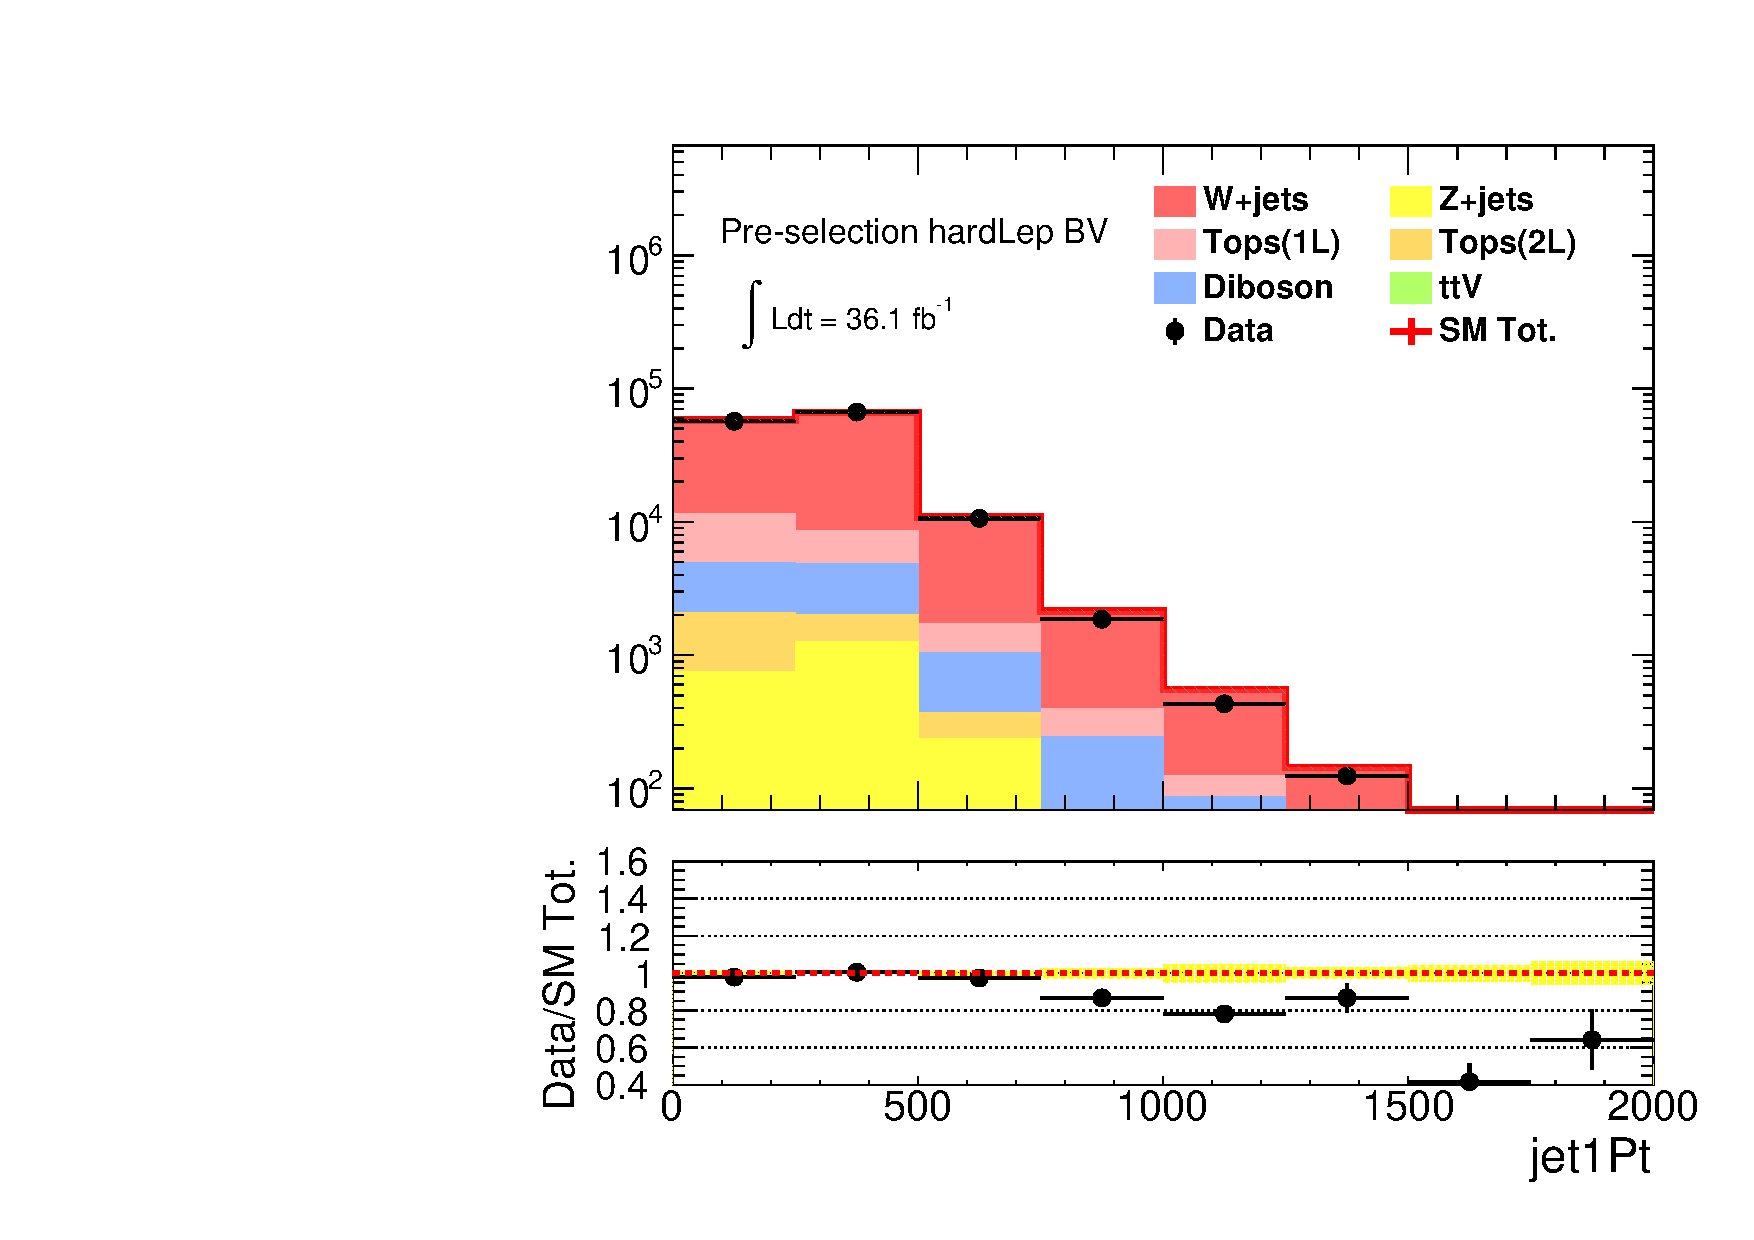
\includegraphics[width=0.48\textwidth]{figures/BGestimation/DataMCComparison/Preselection_hardLepBV/jet1Pt__Preselection_hardLepBV__rwgt_nJ007_ttPt007.pdf}}
    \subfigure[]{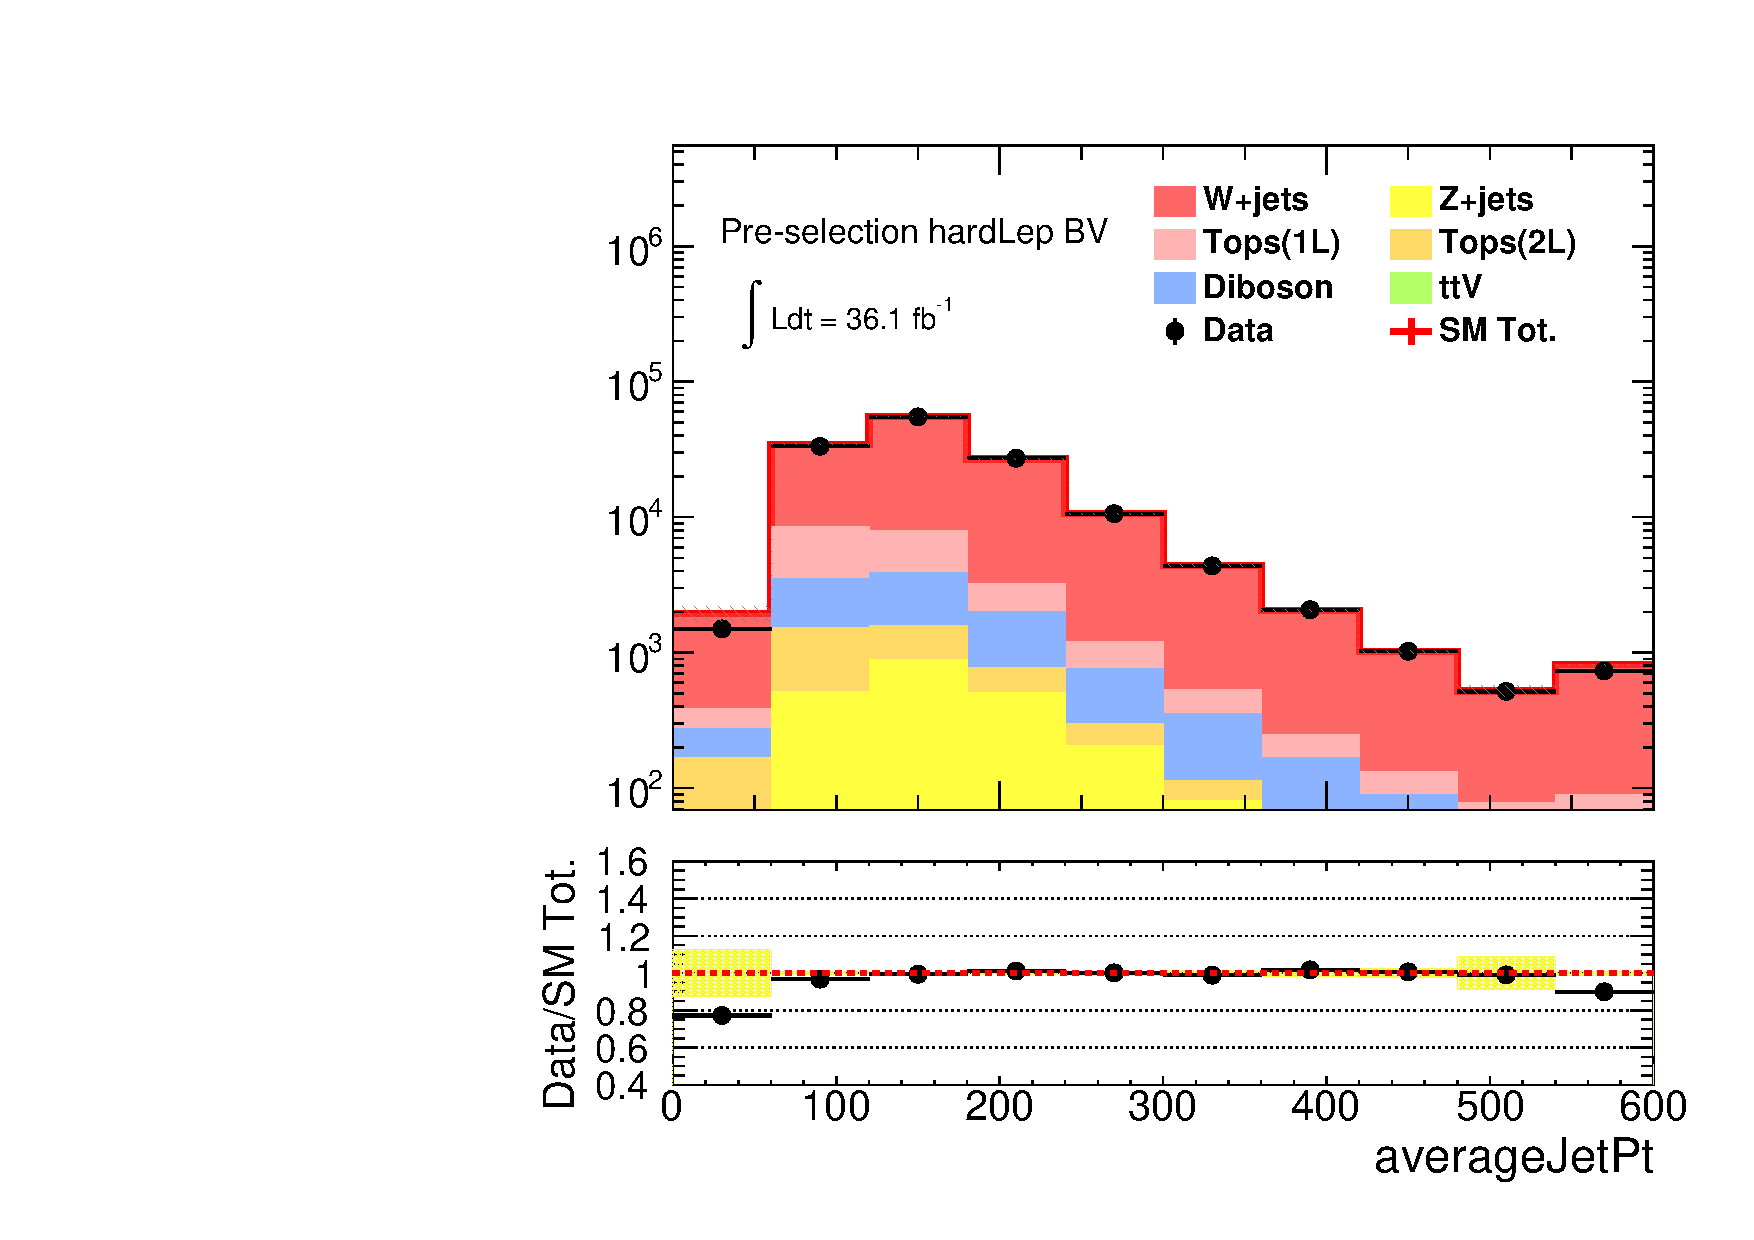
\includegraphics[width=0.48\textwidth]{figures/BGestimation/DataMCComparison/Preselection_hardLepBV/averageJetPt__Preselection_hardLepBV__rwgt_nJ007_ttPt007.pdf}}
    \subfigure[]{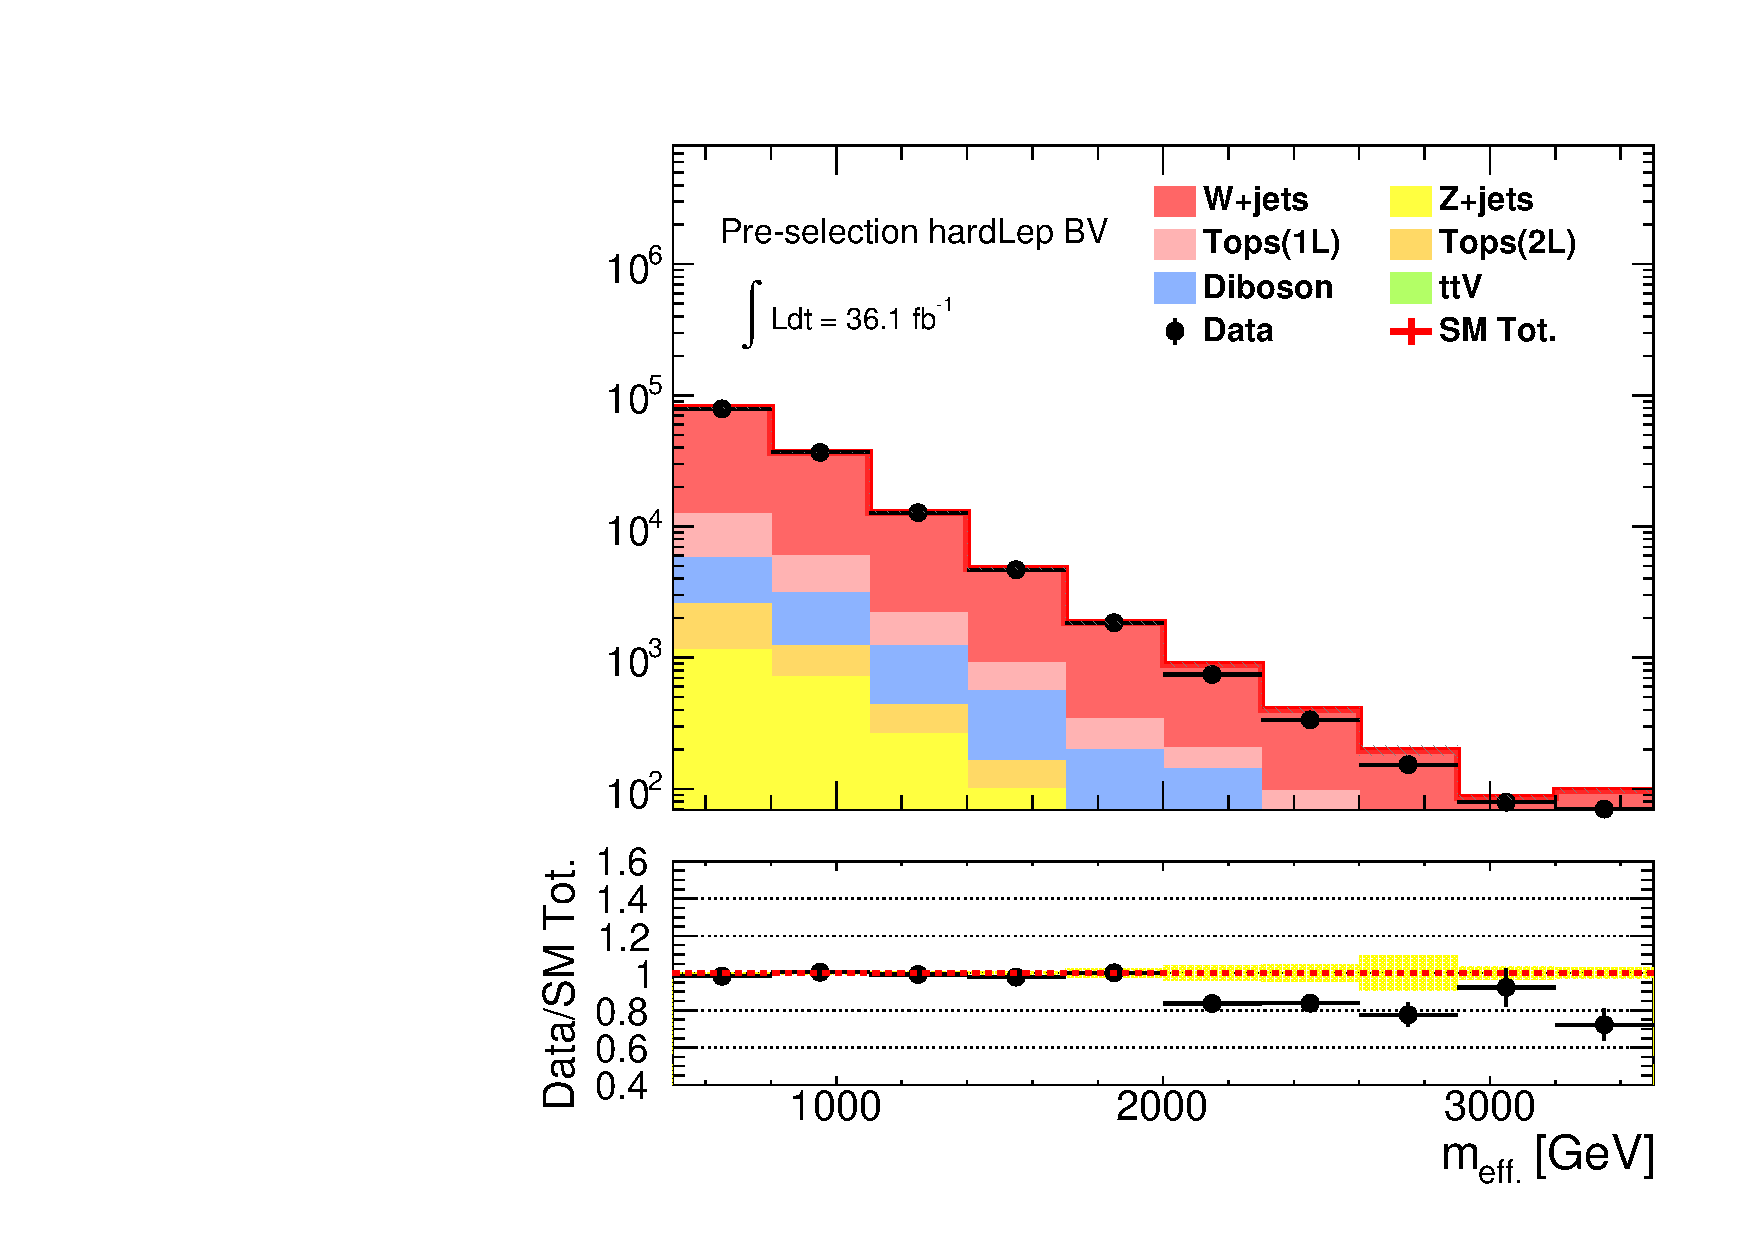
\includegraphics[width=0.48\textwidth]{figures/BGestimation/DataMCComparison/Preselection_hardLepBV/meffInc30__Preselection_hardLepBV__rwgt_nJ007_ttPt007.pdf}}
    \caption{ Kinematical distribution of (a) Jet multiplicity ($p_T>30\gev$) (b) leading-jet pt  (c) average jet pt ($p_T>30\gev$)  (d) $\meffInc$ in the hard lepton b-vetoed pre-selection region, with the reweighting $w = 1 - 0.1 \times (\nJetNoGev-2)$ (Eq.(\ref{eq::BGestimation::rwgt_nJ})) being applied for $\wjets$ MC. 
 \label{fig::BGestimation::DataMCPreselHardBV_rwgt1} }

\end{figure}

\begin{figure}[h]
  \centering
    \subfigure[]{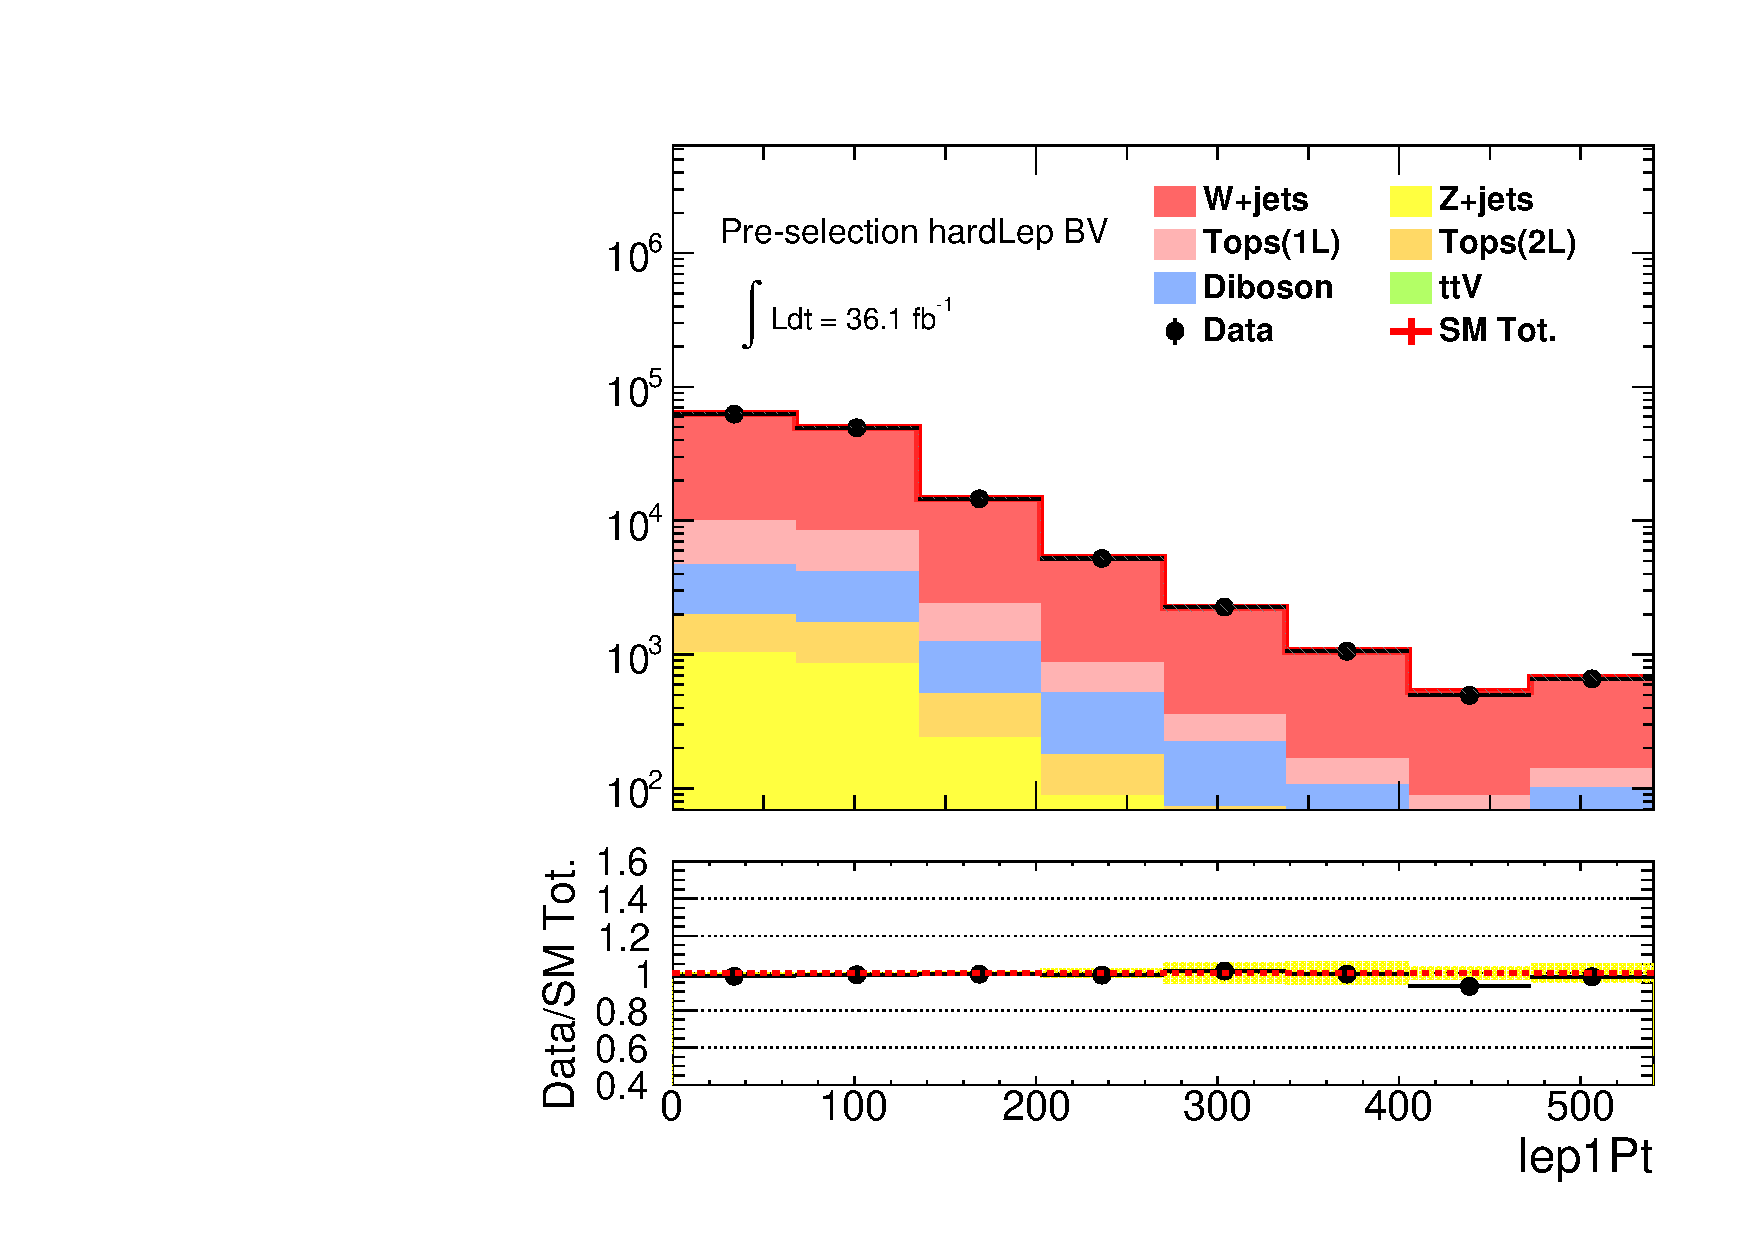
\includegraphics[width=0.48\textwidth]{figures/BGestimation/DataMCComparison/Preselection_hardLepBV/lep1Pt__Preselection_hardLepBV__rwgt_nJ007_ttPt007.pdf}}
    \subfigure[]{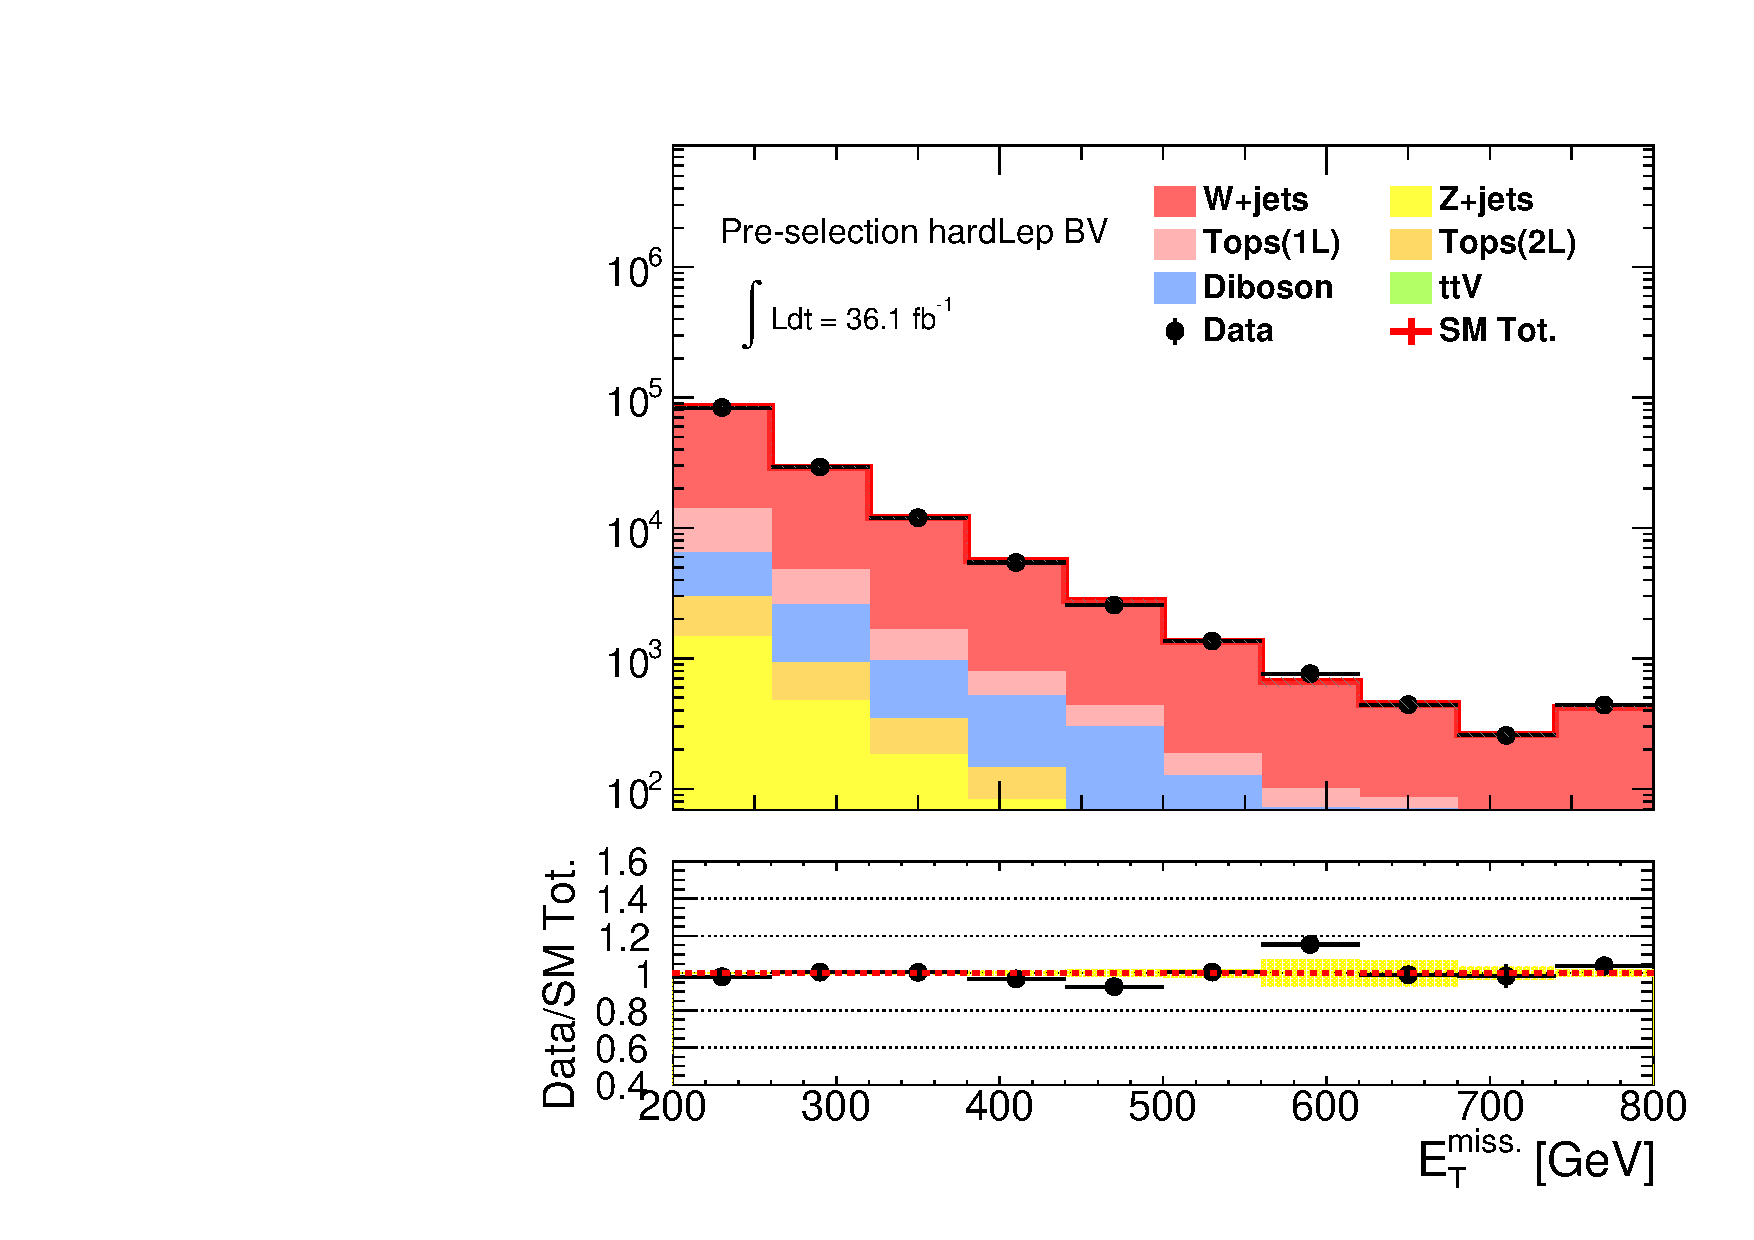
\includegraphics[width=0.48\textwidth]{figures/BGestimation/DataMCComparison/Preselection_hardLepBV/met__Preselection_hardLepBV__rwgt_nJ007_ttPt007.pdf}}
    \subfigure[]{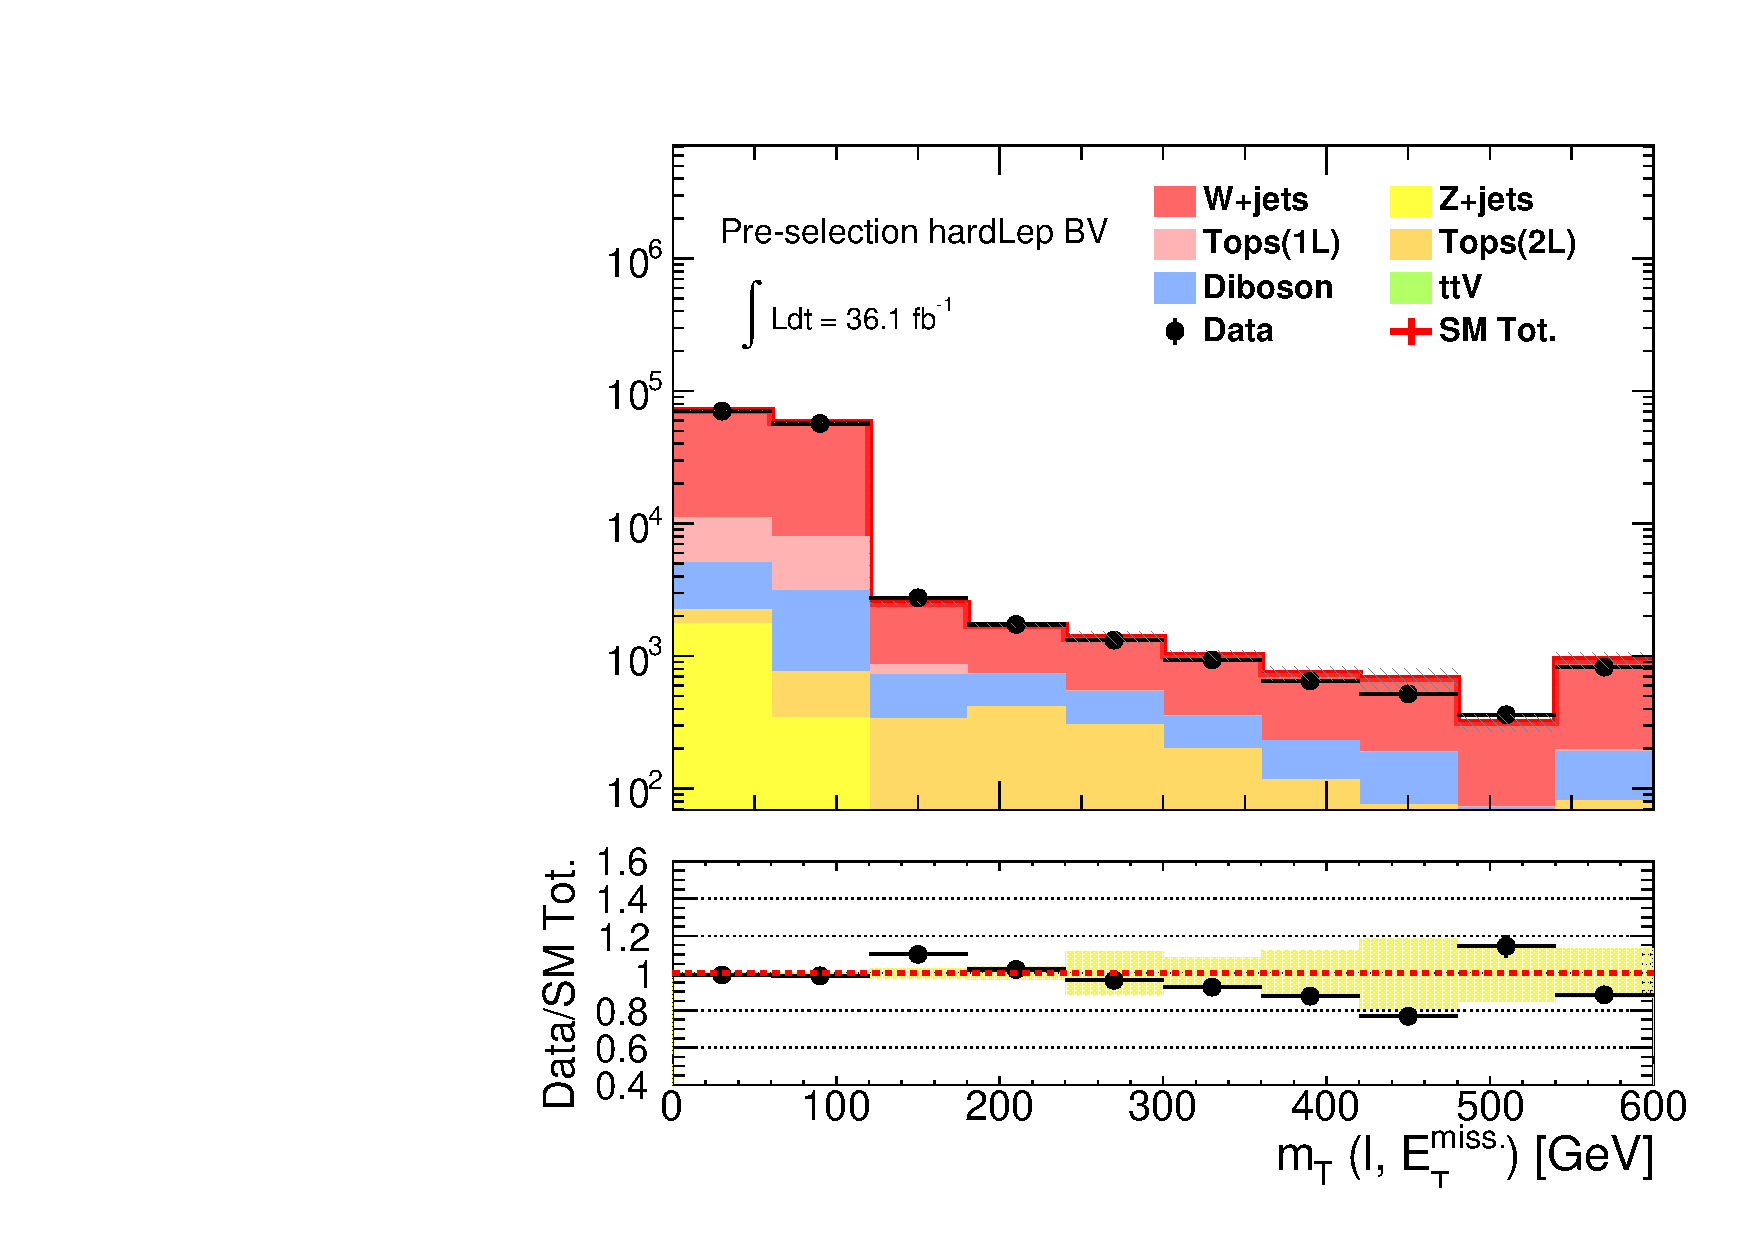
\includegraphics[width=0.48\textwidth]{figures/BGestimation/DataMCComparison/Preselection_hardLepBV/mt__Preselection_hardLepBV__rwgt_nJ007_ttPt007.pdf}}
    \subfigure[]{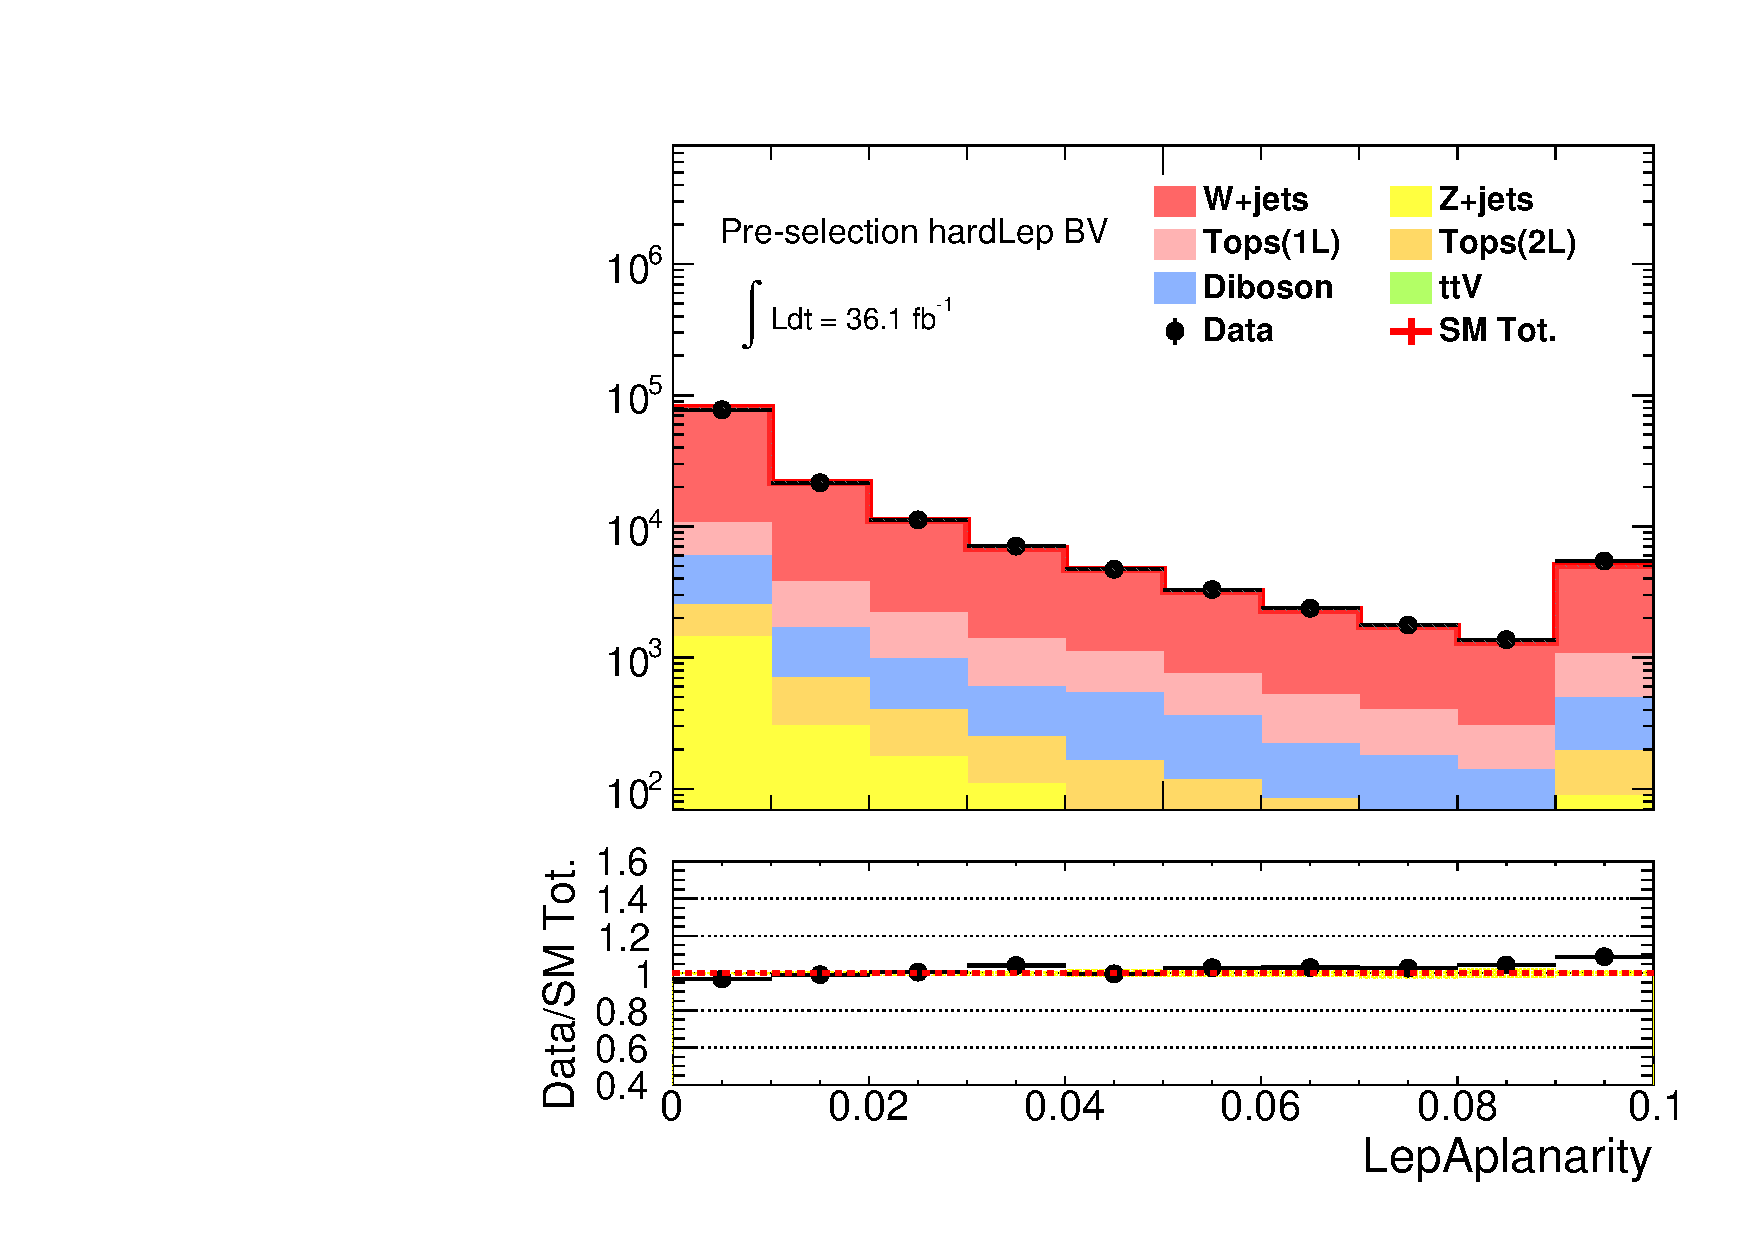
\includegraphics[width=0.48\textwidth]{figures/BGestimation/DataMCComparison/Preselection_hardLepBV/LepAplanarity__Preselection_hardLepBV__rwgt_nJ007_ttPt007.pdf}}
    \caption{ Kinematical distribution of (a) leading-lepton pt (b) $\met$  (c) $\mt$  (d) $\apl$ in the \textbf{hard lepton b-vetoed} pre-selection region, with the reweighting $w = 1 - 0.1 \times (\nJetNoGev-2)$ (Eq.(\ref{eq::BGestimation::rwgt_nJ})) being applied for $\wjets$ MC.  \label{fig::BGestimation::DataMCPreselHardBV_rwgt2} }
\end{figure}

